\chapter{Diseño e implementaci\'on del sistema}

\section{Requerimientos}

Antes del diseño del dispositivo es necesario considerar los siguientes requerimientos de hardware y software.

\subsubsection{Requerimientos de hardware}

\begin{enumerate}
	\item El dispositivo debe incluir un transceptor inalámbrico de 2.4 GHz que cumpla con los estándares IEEE 802.15.4 y ZigBee, 
	\item El dispositivo contará con una interfaz RS-232 para la comunicación serial hacia la computadora embebida, 
	\item El dispositivo deberá contar con un microcontrolador soportado por la pila de desarrollo Atmel BitCloud,
	\item El dispositivo, al funcionar junto a la computadora embebida, deberá compartir la misma fuente de alimentación, razón por la cual el rango de voltaje de operación deberá ser congruente al voltaje de operación de la computadora embebida, 
	\item Se debe considerar la disponibilidad de puertos de expansión para la conexión de sensores y otros dispositivos, 
\end{enumerate}

\subsubsection{Requerimientos de software}

\begin{enumerate}
	\item Se requiere que el dispositivo gestione una WSN, transfiera mensajes desde la WSN hacia el exterior y env\'ie comandos de configuraci\'on hacia los dem\'as dispositivos en la red, 
	\item El dispositivo debe transmitir mediante la interfaz RS-232 la información generada por los nodos en la red, 
	\item Debe ser posible enviar comandos de control hacia los nodos en la red.
\end{enumerate}

\section{Diseño del hardware}

El diseño del dispositivo se centra en el microcontrolador ATmega128RFA1\cite{dev:mega128rfa1}, ver figura \ref{fig:esquematico_completo}. Este dispositivo programable integra un microcontrolador de 8 bits con un radio transceptor de baja potencia de 2.4 GHz en banda ISM con capacidad de funcionamiento dentro de los estándares IEEE 802.15.4 y ZigBee. Sus características principales son : 

\begin{itemize}
	\item Microcontrolador AVR de 8 bits de baja potencia y alto desempeño, 
	\item Arquitectura RISC avanzada,
	\item Memorias no volátiles de datos y programa, 
	\item Interfaz de programación y depuración JTAG (\textit{Joint Test Action Group}),
	\item Periféricos:
	\begin{itemize}
		\item Múltiples contadores, temporizadores y canales PWM, 
		\item Conversor analógico--digital de 10 bits a 330 kS/s, comparador analógico y sensor de temperatura integrado,
		\item Interfaz SPI Maestro/Esclavo, 
		\item Dos unidades USART, 
	\end{itemize}
	\item Transceptor integrado de 2.4 GHz para banda ISM de baja potencia,
	\item 38 líneas I/O programables,
	\item Voltaje de alimentación de $ 1.8 - 3.6\,Vcd $,
	\item Consumo de potencia:
	\begin{itemize}
		\item CPU modo activo (16 MHz) : $4.1\,mA$, 
		\item Transceptor 2.4 GHz : RX\_ON $12.5\,mA$ / TX $14.5\,mA$, 
		\item Modo de bajo consumo : $<250\,nA\; @\; 25\,^{\circ}\mathrm{C}$
	\end{itemize}
\end{itemize}

La arquitectura de este microcontrolador permite simplificar el diseño general del dispositivo. Al tener el radio transceptor integrado se reduce el número de componentes externos y en consecuencia se disminuye el espacio físico y el consumo de energía. De la misma forma, se incrementa la velocidad de transferencia de datos entre el radio transceptor y los demás componentes internos. 

El microcontrolador ATmega128RFA1 es compatible con diversos compiladores, depuradores y herramientas de programación. En particular, Atmel BitCloud soporta la arquitectura de este microcontrolador para el desarrollo de aplicaciones de WSN.

\begin{landscape}

\begin{figure}
	\includegraphics[scale=0.8]{capitulo_3_imgs/esquematico_completo.pdf}
	\caption{Diseño de circuito esquem\'atico del dispositivo}
	\label{fig:esquematico_completo}

\end{figure}

\end{landscape}

\subsection{Antena}

La implementación de la radio comunicación se realizó con una antena ANT-2.4-CHP de 2.4 GHz de amplio ancho de banda y baja pérdida\cite{dev:antena}. La sección del diagrama del circuito se muestra en la figura \ref{fig:esquematico_antena}. Con esta antena, identificada en el diagrama como \textit{ANTENNA2SMD5}, se simplifica la implementación de la radio comunicación al requerir un mínimo de componentes adicionales para el filtrado y protección de los componentes del circuito. 

\begin{figure}
	\centering
	\includegraphics[scale=0.8]{capitulo_3_imgs/esquematico_antena.pdf}
	\caption{Antena del circuito}	
	\label{fig:esquematico_antena}
\end{figure}

\subsection{Fuente de energía}

Se consideran dos factores en el diseño de la fuente de alimentación del dispositivo: 1) la fuente de alimentación externa se compartirá con la computadora industrial, cuyo rango de voltaje es de 12 -- 48 Vcd y 2) que el rango de voltaje de operación del microcontrolador es de 1.8 -- 3.6 Vcd, utilizando 3.3 Vcd como voltaje central. Por lo tanto se requiere de un regulador de voltaje de 3.3 Vcd con un amplio rango de voltaje de operación. 

La fuente de enegía se implementó con el regulador de voltaje LF33AB\cite{dev:regulador}. Este regulador tiene un rango de operación de 3.3 -- 16 Vcd y entrega un voltaje de salida fijo de 3.3 Vcd limitando la corriente a un máximo de 500 mA. 

En el diagrama mostrado en la figura \ref{fig:esquematico_fuente} se observa la implementación de la fuente de energía. Se habilitaron dos conectores para la alimentación del voltaje, \textit{J1} y \textit{JP1}, que permite la conexión mediante un \textit{Jack} estándar o dos cabezales de 0.1 pulgadas respectivamente. De esta forma el dispositivo puede ser alimentado con una gran variedad de fuentes de energía. 

\begin{figure}
	\centering
	\includegraphics[scale=0.8]{capitulo_3_imgs/esquematico_fuente.pdf}
	\caption{Regulador de voltaje del circuito}	
	\label{fig:esquematico_fuente}
\end{figure}

\subsection{Puertos de comunicaci\'on}

La comunicación serial entre el dispositivo y la computadora industrial se realiza mediante el estándar RS-232. Este estándar define las características eléctricas y de sincronización de las señales para el intercambio de datos binarios entre equipos, conectados a través de cableado y conectores definidos en el estándar. 

Sin embargo, RS-232 no contempla aspectos como la estructura e integridad de los datos. Para ello, el módulo USART (\textit{Universal Synchronous/Asynchronous Receiver/Transmitter}) inmerso en el microcontrolador es el encargado de ofrecer una interfaz entre los registros internos del microcontrolador y la comunicación serial. 

\begin{figure}
	\centering
	\includegraphics[scale=0.8]{capitulo_3_imgs/esquematico_max232.pdf}
	\caption{Puerto de comunicaci\'on serial RS-232}
	\label{fig:esquematico_max232}
\end{figure}

En una configuración típica de conexión entre un microcontrolador y otro equipo mediante el estándar RS-232, es necesario acondicionar los niveles de voltaje de la señal emitida por la USART para que sean compatibles con RS-232. En la figura \ref{fig:esquematico_max232} se muestra la implementación de la comunicación serial RS-232. Se utilizó un acondicionador de señal MAX3232\cite{dev:max3232} que nivela el voltaje de las señales de la USART de 3.3 Vcd a 5.5 Vcd; nivel de voltaje reconocible por RS-232. 

El dispositivo dispone de dos enlaces físicos para la comunicación serial (\textit{X1} y \textit{JP2} en el diagrama), un conector DB9 hembra para la conexión directa hacia la computadora industrial y tres terminales de 0.1 pulgadas para otros dispositivos.   



\subsubsection{Puertos adicionales}

\begin{figure}
	\centering
	\includegraphics[scale=0.8]{capitulo_3_imgs/esquematico_puertos.pdf}
	\caption{Puertos de comunicación adicionales}
	\label{fig:esquematico_puertos}
\end{figure}

Se habilitaron 23 puertos multipropósito en el dispositivo para programación, depuración de programas y comunicación con sensores y otros dispositivos, ver figura \ref{fig:esquematico_puertos}. Se incorporó un puerto JTAG para cargar y depurar programas en el microcontrolador, asi como un puerto SPI (\textit{Serial Peripheral Interface}) para la comunicación serial mediante este protocolo. Adicionalmente se agregaron tres LEDs indicadores (rojo, verde y amarillo) para generar mensajes visuales. En la tabla \ref{tabla:puertos} se muestra el resumen de puertos disponibles en el dispositivo. 

\begin{table}
	\begin{center}
		\caption{Puertos del microcontrolador disponibles en el circuito}
		\label{tabla:puertos}
		\small
		\begin{tabular}{l|c}
			\toprule
			\textbf{Puerto} & \textbf{Cantidad}\\
			\midrule
			Entradas al conversor analógico--digital & 7\\
			Salidas PWM & 7\\
			Entradas de interrupciones externas & 9\\
			Programación y depuración JTAG & 1\\
			Comunicación SPI & 1\\
			\bottomrule
		\end{tabular}
	\end{center}
\end{table}

\subsection{Diseño de circuito impreso}

Se realizó el diseño PCB (\textit{Printed Circuit Board}) de dos capas con dimensiones de 60 mm de ancho por 78 mm de largo. A la izquierda de la figura \ref{fig:circuito_fabricado} se muestra el diseño PCB. Este diseño de compone de varias capas que separan la cara superior, la cara inferior, las perforaciones en la tarjeta y el texto o figuras que se imprimen. Esta información es utilizada para la manufactura y ensamble del circuito. A la derecha de la figura \ref{fig:circuito_fabricado} se muestra el circuito fabricado. 

\begin{figure}
	\centering
	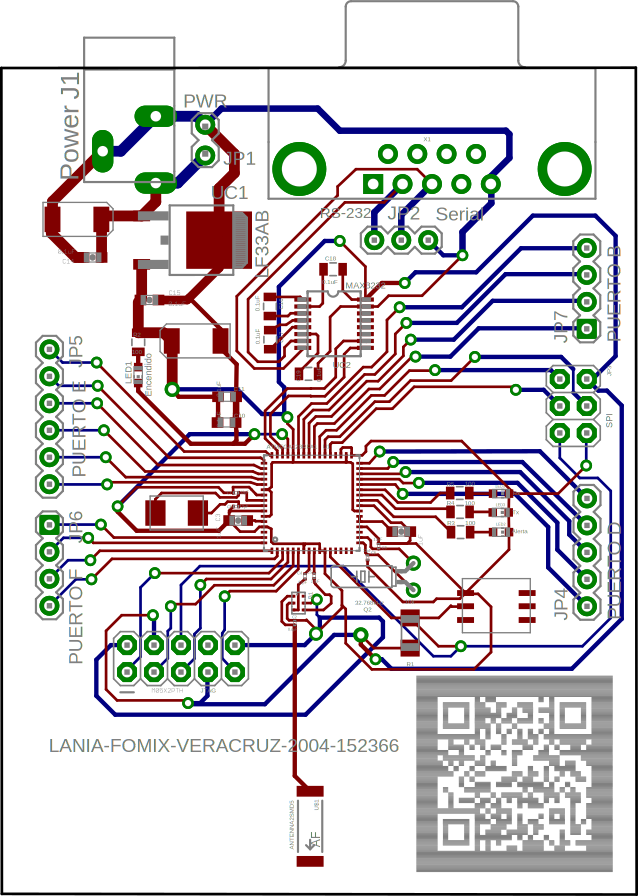
\includegraphics[scale=0.4]{capitulo_3_imgs/diseno_pcb.pdf}
	\caption{Diseño de circuito impreso}
	\label{fig:circuito_fabricado}
\end{figure}

\section{Diseño del software}

%El diseño del software embebido para el dispositivo se divide en cuatro partes principales. En primer lugar, considerando que el dispositivo responderá a comandos enviados desde la interfaz RS-232, se eligieron los comandos básicos para la gestión de una WSN. Posteriormente se diseña un protocolo de comunicación para transferir mensajes y datos entre el dispositivo y la computadora embebida. En tercer lugar, se implementa el software embebido que interpreta los mensajes empaquetados en la estructura del protocolo y ejecuta su acción correspondiente. Por último, se diseñan e implementan un conjunto de funciones para hacer uso del dispositivo desde la computadora embebida industrial. 

\subsection{Protocolo de comunicación}

Se diseñó un protocolo de comunicación para la transferencia bidireccional de comandos y mensajes de datos entre la computadora embebida y el dispositivo mediante la interfaz RS-232. En este protocolo la información se transmite en paquetes de datos con la estructura mostrada en la figura \ref{fig:protocolo}, donde cada campo se define de la siguiente manera : 

\begin{itemize}
	\item \textit{Delimitadores} : El inicio y fin de cada trama de datos está marcado por bytes delimitadores; el byte delimitador inicial tiene un valor fijo de 0x55 mientras que el byte delimitador final tiene un valor de 0xAA.	
	\item \textit{Longitud de trama} : Este campo de dos bytes especifica el número de bytes que contiene la trama, incluyendo los bytes de control y delimitadores. La longitud mínima de la trama es de 6 bytes, mientras que el máximo es de 65536 bytes. Este campo permite conocer la posición del delimitador final para comprobación de errores, 
	\item \textit{Identificador de mensaje} : Campo de un byte que le permite al usuario asignar a cada comando un número de identificación único. La respuesta asociada a cada comando contendrá este mismo identificador,
	\item \textit{Comando} : Campo de un byte que contiene el identificador del comando o mensaje contenido dentro de la trama,
	\item \textit{Datos o parámetros} : En este campo opcional de longitud variable se incluyen los parámetros requeridos por algunos comandos así como datos de respuesta. 
\end{itemize}

\begin{figure}
	\centering
	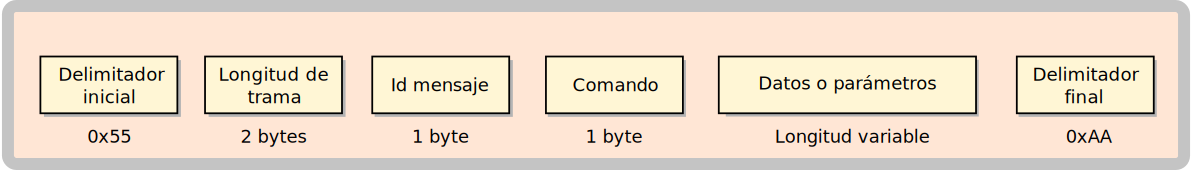
\includegraphics[scale=0.4]{capitulo_3_imgs/protocolo.pdf}
	\caption{Definición de trama del protocolo de comunicación}
	\label{fig:protocolo}
\end{figure}

La tabla \ref{tabla:lista_comandos} muestra un resumen de los comandos, su clasificación y respuestas asociadas. Los comandos dentro de la categoría de \textit{Información de la red} se encargan de obtener información sobre el estado de la red inalámbrica, el número y direcciones de los nodos conectados y la calidad de los enlaces de radio comunicación. Los comandos dentro de la categoría \textit{Transferencia de datos} se encargan de transferir información hacia un nodo o un grupo de nodos en la red. 

Así mismo, se definió el conjunto de comandos \textit{Gestión de nodos} para configurar el modo de operación de cada nodo. Para esto se considera que los nodos dentro de la WSN funcionarán en alguno de estos tres modos de operación: 

\begin{enumerate}
	\item \textit{Modo Solicitud--Respuesta} : En este modo el nodo siempre está activo esperando solicitudes de datos desde el coordinador de la red, en este modo se presenta el mayor consumo de energía,  
	\item \textit{Modo de ahorro de energía} : Este modo consiste en la desactivación periódica de todos los componentes de hardware del nodo. Al terminar cada periodo el nodo se activa para recolectar información sensorial y transmitirla hacia el coordinador de la red. 
	\item \textit{Modo de ahorro de energía parcial} : Este modo sólo los componentes de radio frecuencia se desactivan periódicamente. Esto permite que el nodo pueda realizar otras tareas mientras no esté transmitiendo datos a la red. 
\end{enumerate}

De la misma forma se definió un comando en la categoría de \textit{Lectura de sensores} para transferir información de los sensores conectados directamente al dispositivo. Por último se definieron mensajes de respuesta en caso de errores en la estructura y parámetros de cada comando, estos mensajes se encuentran en la categoría \textit{Respuestas de control} también mostrada en la tabla \ref{tabla:lista_comandos}. La lista completa de comandos y mensajes de datos se encuentra en el anexo \textit{Comandos y mensajes de datos}.

\begin{table}
	\begin{center}
	\caption{Conjunto de comandos básicos de control de una WSN}
	\label{tabla:lista_comandos}
	\small
	\begin{tabular}{c|l|l}
		\toprule
		\textbf{Tipo} & \textbf{Comando} & \textbf{Respuesta}\\ % & \textbf{Descripción}\\
		\midrule
		\multirow{5}{*}{\textbf{Información sobre la red}} & DEVICE\_STATUS & DEVICE\_UP\\ 
		%\cline{2-3} 
		& \multirow{2}{*}{GET\_NETWORK\_STATUS} & IN\_NETWORK\_STATUS\\ & & OUT\_NETWORK\_STATUS\\ 
		%\cline{2-3}
		& GET\_CHILDREN\_AMOUNT & CHILDREN\_AMOUNT\\ % & Obtiene el número de nodos conectados a la red inalámbrica.\\
		& GET\_CHILDREN\_LIST & CHILDREN\_LIST\\ % & Obtiene las direcciones de red de los nodos conectados a la red inalámbrica.\\
		& GET\_LQI\_RSSI & LQI\_RSSI\\ % & Obtiene los valores RSSI y LQI respecto a un nodo específico.\\
		\midrule
		\multirow{3}{*}{\textbf{Transferencia de datos}} & 
		DATA\_FROM\_NODE\\ 
        & SEND\_DATA\_NODE & DATA\_SENT\\ % & Envía datos a un nodo específico\\
		& SET\_RECV\_NODE & DATA\_RECEPTION\_CHANGED\\ % & Habilita la transmisión de datos desde la red mediante la interfaz RS-232\\
		\midrule
		\multirow{4}{*}{\textbf{Gestión de nodos}} &
		SET\_NODE\_OP\_MODE & MODE\_SET\\ % & Establece el modo de operación de un nodo\\
		& START\_SLEEP\_NODE & MODE\_STARTED\\ % & Inicia el modo de inactividad en un nodo específico\\
		& STOP\_SLEEP\_MODE & MODE\_STOPED\\
		& START\_RF\_MODE & MODE\_STARTED\\ % & Inicia el modo de inactividad de la radio en un nodo específico\\
		& STOP\_RF\_MODE & MODE\_STOPED\\
		& REQUEST\_DATA\_NODE & DATA\_REQUEST\\ % & Adquisición de datos de un nodo específico\\
		\midrule
		\textbf{Lectura de sensores} & 
		READ\_SENSORS & SENSOR\_DATA\\ % & Obtiene datos los sensores conectados al circuito\\
		\midrule 
		\multirow{3}{*}{\textbf{Respuestas de control}} &
		UNKNOWN\_COMMAND\\
		& BAD\_PARAMETERS\\
		& INCORRECT\_MSG\_SIZE\\
		\bottomrule
		\end{tabular}
	\end{center}
\end{table}

\subsubsection{Ejemplo de transferencia de comandos}

En este ejemplo se muestra la transferencia de mensajes para la ejecución del comando GET\_NETWORK\_STATUS dentro de la categoría \textit{Información de la red}. Este comando permite conocer si la red inalámbrica ha sido iniciada por el dispositivo y de ser así devuelve el identificador de la red en un número de 16 bits. En el anexo \textit{Comandos y mensajes de datos} se puede observar un mayor detalle sobre este comando. 

GET\_NETWORK\_STATUS (código : 0x02) tiene dos respuestas asociadas. Cuando la red se ha iniciado devuelve el mensaje IN\_NETWORK\_STATUS (código : 0x58) junto con dos bytes conteniendo el identificador de la red, en caso contrario, se recibe el mensaje OUT\_NETWORK\_STATUS (código : 0x59). 

En la figura \ref{fig:protocolo_ejemplo} se muestran las tramas de datos del comando y de sus dos respuestas asociadas. En la parte superior se muestra el comando enviado hacia el dispositivo. Esta trama de 6 bytes transfiere el código de comando 0x02 y los bytes de longitud marcan la longitud de toda la trama (0x0006). El campo de identificador de mensaje se ha definido arbitrariamente en este ejemplo con un valor de 0x01.

La primera respuesta devuelve una trama compuesta por 8 bytes, en este caso se devolvió el código de mensaje 0x58 y dos bytes adicionales para la dirección de red con un valor 0x01f3 para este ejemplo. Por último, la segunda respuesta devuelve el valor 0x59 sin datos adicionales, por lo que el tamaño de la trama es de 6 bytes. En estas dos respuestas el identificador de mensaje es devuelto de la misma forma que ha sido definido en el comando inicial.   

 
\begin{figure}
	\centering
	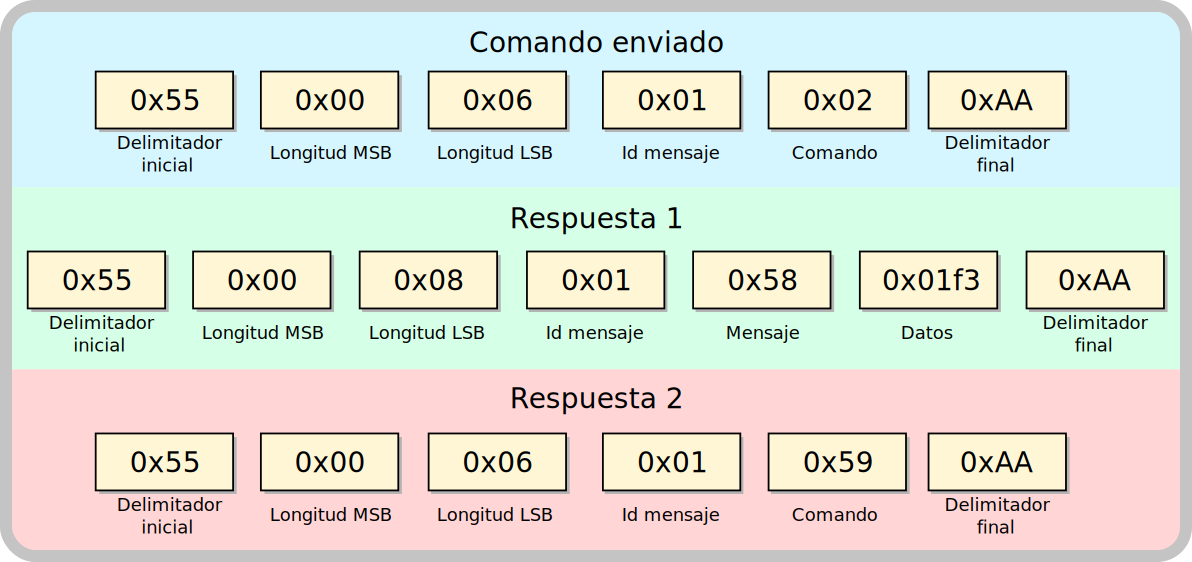
\includegraphics[scale=0.4]{capitulo_3_imgs/protocolo_ejemplo_1.pdf}
	\caption{Ejemplo de uso de protocolo de comunicación}
	\label{fig:protocolo_ejemplo}
\end{figure}

\subsection{Implementación de software embebido}

\begin{figure}
	\centering
	\includegraphics[scale=1.2]{capitulo_3_imgs/app_sd.pdf}
	\caption{Software embebido del dispositivo como máquina de estados}
	\label{fig:maquina_estados_sd}
\end{figure}

Para el software embebido del dispositivo se desarrolló una aplicación de BitCloud que se encarga de recibir mensajes y/o comandos desde la interfaz RS-232, validar que la información recibida esté estructura en términos del protocolo de comunicación diseñado y por último, implementar la funcionalidad de cada uno de los comandos, utilizando para esto las funciones que provee BitCloud para el control de periféricos y de la red inalámbrica. En la figura \ref{fig:maquina_estados_sd} se puede ver a la aplicación representada como una máquina de estados los cuales son detallados a continuación. 

\begin{figure}
	\centering
	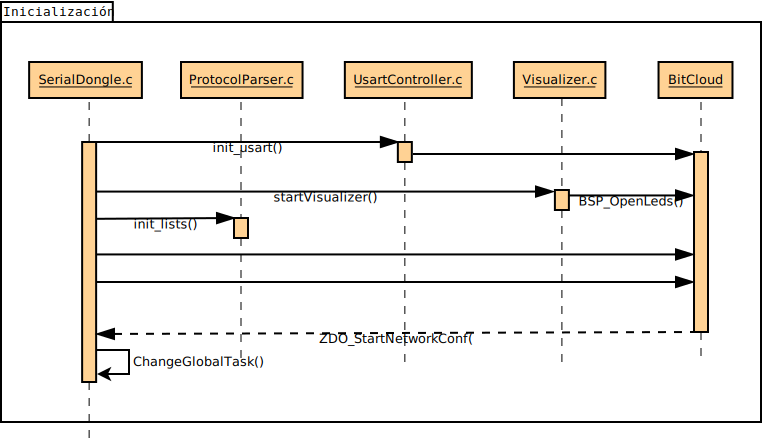
\includegraphics[scale=0.35]{capitulo_3_imgs/Inicializacion.pdf}
	\caption{Inicialización de la aplicación}
	\label{fig:diagrama_inicializacion}
\end{figure}

\subsubsection{Inicialización}

Al iniciar la aplicación, ver figura \ref{fig:diagrama_inicializacion}, las función init\_usart() es llamada para configurar el puerto serial mediante el control de periféricos que provee BitCloud, asi mismo se configuran los puertos para los LEDs indicadores de la tarjeta. Posteriormente se inicializan las colas de almacenamiento de mensajes que se detallaran más adelante. 

La aplicación se registra en BitCloud utilizando un identificador (\textit{end point}) único en la red, y con esta información se solicita el inicio de la red a BitCloud. Al terminar esta solicitud la función asíncrona ZDO\_StartNetworkConf() es llamada y realiza el cambio de estado de la aplicación. 

\begin{figure}
	\centering
	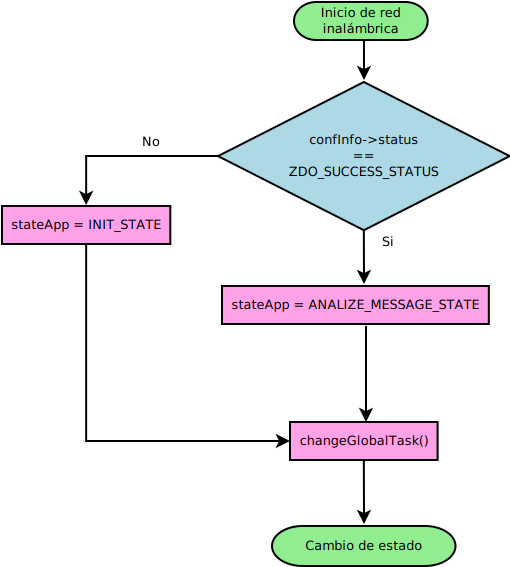
\includegraphics[scale=0.35]{capitulo_3_imgs/inicio_red.pdf}
	\caption{Inicio de la red inalámbrica}
	\label{fig:diagrama_inicio_red}
\end{figure}

\subsubsection{Inicio de la red inalámbrica}

En este estado se analiza el resultado de la operación de BitCloud para el inicio de la red inalámbrica. Si el resultado es ZDO\_SUCCESS\_STATUS entonces la red inalámbrica ha sido iniciada correctamente y el dispositivo está listo para iniciar su operación pasando al estado de \textit{Esperar comandos y/o mensajes}, de lo contrario el dispositivo vuelve al estado de \textit{Inicialización} del dispositivo. En la figura \ref{fig:diagrama_inicio_red} se muestra el diagrama de flujo de este estado.


\subsubsection{Esperar comandos y/o mensajes}

En este estado la aplicación espera por comandos enviados desde el puerto serial, la figura \ref{fig:interprete_mensajes} muestra un diagrama de bloques con los distintos elementos de este estado. La información recibida es validada y desempaquetada por el \textit{intérprete de protocolo} para luego ser almacenada en la cola de comandos entrante, posteriormente el \textit{intérprete de comandos} valida el comando especificado. Cada comando es ejecutado y su resultado es almacenado en la cola de mensajes salientes. Por último la información es enviada por la interfaz serial en la estructura del protocolo de comunicación.  

\begin{figure}
	\centering
	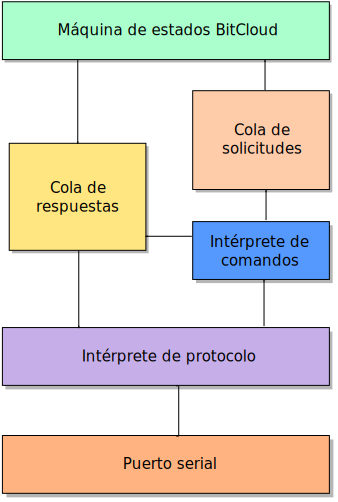
\includegraphics[scale=0.5]{capitulo_3_imgs/estructura_interprete.pdf}
	\caption{Estructura del intérprete de mensajes}
	\label{fig:interprete_mensajes}
\end{figure}

En la figura \ref{fig:diagrama_secuencia_analisis} se detalla la recepción de información por el puerto serial. Cuando un byte es recibido, BitCloud ejecuta la función recv\_bytes() para obtener la información y almacenarla en un buffer temporal. Para poder interpretar la trama recibida es necesario tener por lo menos tres bytes: la cabecera de la trama y los dos bytes de la longitud. Teniendo esta información se han definido dos condiciones para interpretar un inicio de trama válido: 1) que el primer byte tenga el valor de la cabecera (0x55) y 2) que el valor de la longitud sea mayor o igual a 6 bytes, el tamaño de trama mínimo. Si alguna de estas condiciones no se cumple se genera un mensaje de error y se envia por el puerto serial. En la figura \ref{fig:diagrama_flujo_parser} se muestra el diagrama de flujo para el intérprete de protocolo.

Cuando se ha recibido un número de bytes igual a la longitud de la trama entonces se comprueba que el último byte corresponda al final de trama (0xAA). La información restante se desempaqueta de acuerdo a la posisición de cada byte en la trama. Por último se crea una estructura de datos, ver tabla \ref{tabla:s_data_command}, y se agrega esta estructura a la cola de comandos entrante. 

\begin{figure}
	\centering
	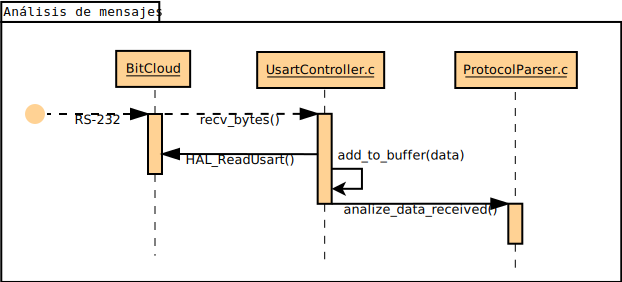
\includegraphics[scale=0.45]{capitulo_3_imgs/analisis_mensajes_secuencia.pdf}
	\caption{Diagrama de secuencia de análisis de mensajes}
	\label{fig:diagrama_secuencia_analisis}
\end{figure}

\begin{figure}
	\centering
	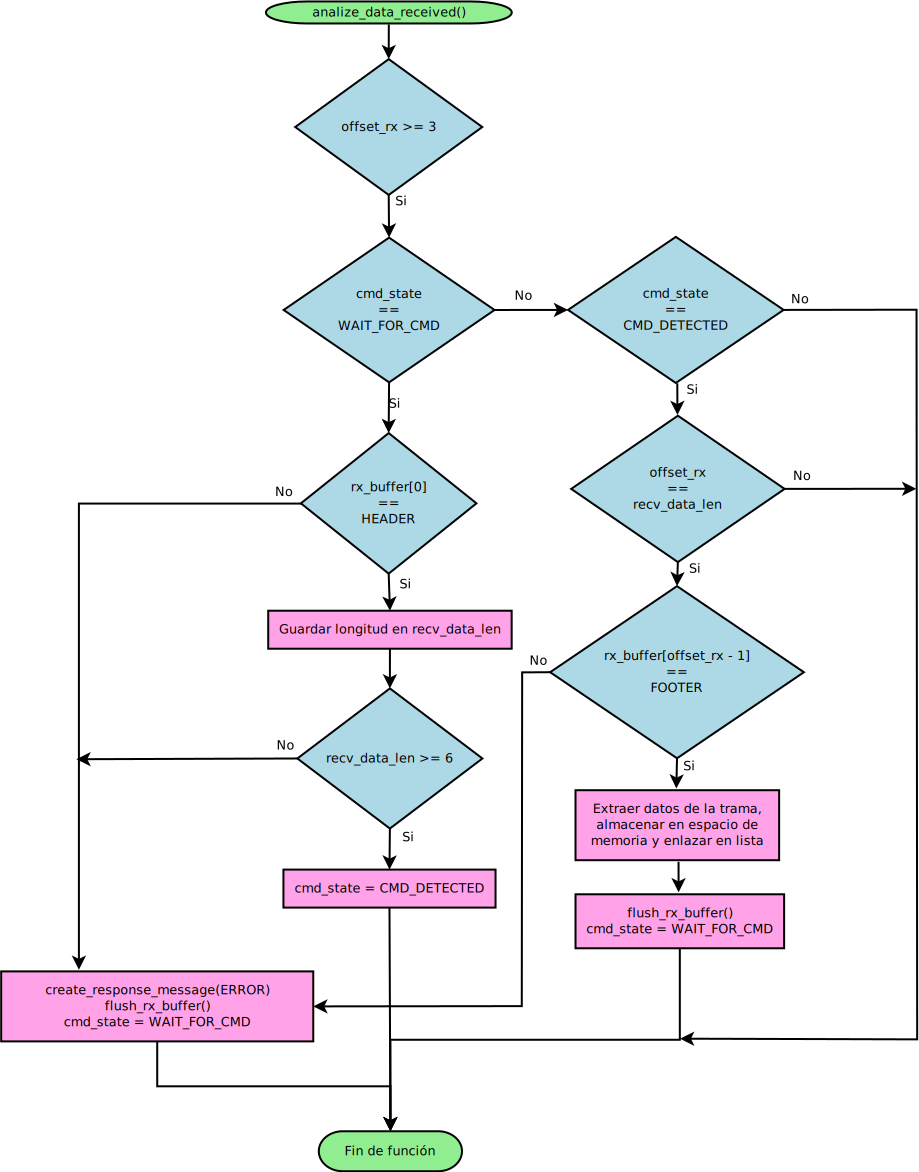
\includegraphics[scale=0.25]{capitulo_3_imgs/analisis_mensaje_flujo_parser.pdf}
	\caption{Diagrama de flujo análisis de protocolo}
	\label{fig:diagrama_flujo_parser}
\end{figure}

Para atender cada comando se verifica el inicio de la cola de comandos entrantes, si hay un elemento en esta cola entonces la aplicación pasa al estado de \textit{Procesar comandos}. Si hay elementos en la cola de mensajes salientes entonces la aplicación pasa al estado de \textit{Enviar mensajes}. La figura \ref{fig:diagrama_flujo_analisis} muestra el digrama de flujo de este estado. 

\begin{table}
	\begin{center}
		\caption{Estructura de datos s\_data\_command}
		\label{tabla:s_data_command}
		\small
		\begin{tabular}{r|l}
			\toprule
			\textbf{Tipo} & \textbf{Variable}\\
			\midrule
			uint8\_t & id\_message \\
			uint8\_t & command \\
			uint8\_t & data\_length \\
			uint8\_t & *data \\
			struct s\_data\_command & *next\_command\\
			\bottomrule
		\end{tabular}
	\end{center}
\end{table}

\begin{figure}
	\centering
	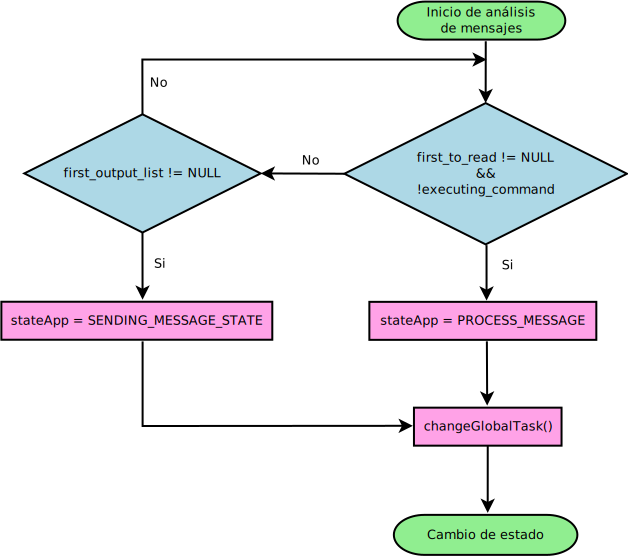
\includegraphics[scale=0.35]{capitulo_3_imgs/analisis_mensajes_flujo.pdf}
	\caption{Diagrama de flujo de análisis de mensajes}
	\label{fig:diagrama_flujo_analisis}
\end{figure}


\subsubsection{Procesamiento de comandos}

En este estado se ejecuta el comando especificado en el primer elemento de la lista de comandos entrantes, ver figura \ref{fig:diagrama_secuencia_procesamiento}. Para esto, el primer elemento de la cola es movido a un espacio temporal a traves de la llamada a move\_first\_to\_execute(). Mediante parse\_command() se ejecuta la función de BitCloud asociada a cada comando y se espera su respuesta. La información recibida es almacenada en la estructura y esta se mueve a la cola de mensajes saliente.

La aplicación pasa al estado \textit{Enviar mensajes} si aún hay elementos disponibles en la lista de mensajes salientes, de lo contrario regresa al estado de \textit{Esperar comandos y/o mensajes} como se detalla en la figura \ref{fig:diagrama_flujo_procesamiento}. 

\begin{figure}
	\centering
	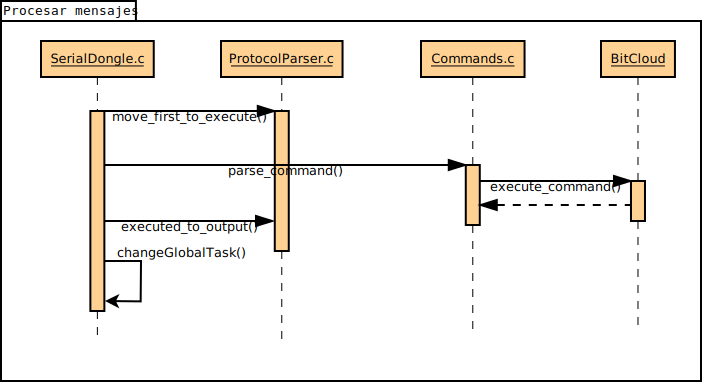
\includegraphics[scale=0.35]{capitulo_3_imgs/procesar_mensajes_secuencia.pdf}
	\caption{Diagrama de secuencia de procesamiento de mensajes}
	\label{fig:diagrama_secuencia_procesamiento}
\end{figure}

\begin{figure}
	\centering
	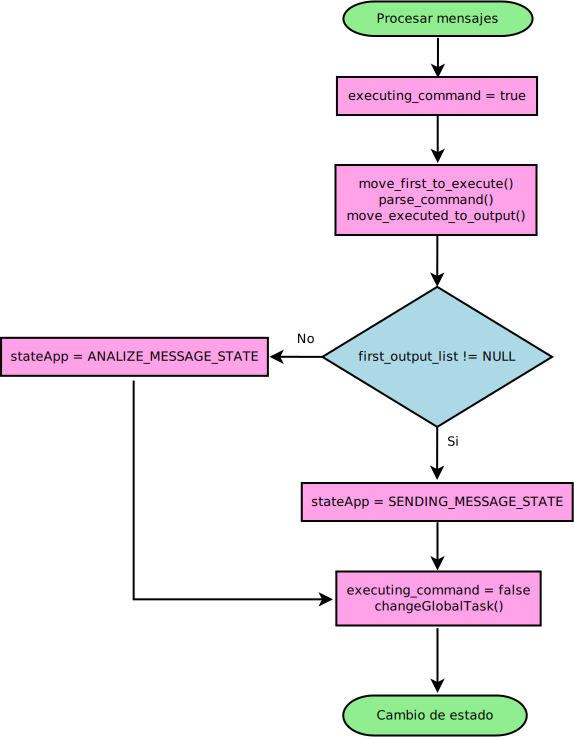
\includegraphics[scale=0.35]{capitulo_3_imgs/procesar_mensaje_flujo.pdf}
	\caption{Diagrama de flujo de procesamiento de mensajes}
	\label{fig:diagrama_flujo_procesamiento}
\end{figure}

\subsubsection{Envío de respuestas}

En este estado se toma el primer elemento de la cola de mensajes salientes, se forma la trama de datos a partir de la información en la estructura de datos y se envía por el puerto serial, ver figura \ref{fig:diagrama_enviar_secuencia}. 

\begin{figure}
	\centering
	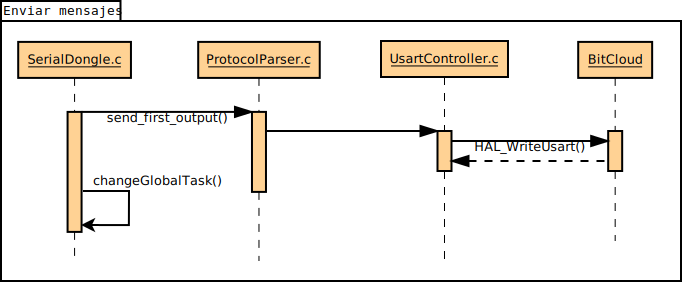
\includegraphics[scale=0.35]{capitulo_3_imgs/enviar_mensajes_secuencia.pdf}
	\caption{Diagrama de secuencia enviar mensajes}
	\label{fig:diagrama_enviar_secuencia}
\end{figure}


\subsection{Programación API MOXA}